\documentclass{beamer}
\usepackage[T1]{fontenc}
\usepackage[utf8x]{inputenc} 
\usepackage[esperanto]{babel}
%\usepackage{umbcboxes}

\title{Komputilsimuladoj}
\subtitle{Ĉelaŭtomatoj}
\author{Tomasz Szymula}
\institute[PEJ]{Pola Esperanto-Junularo}

\date[JES 2013]{Junulara Esperanto-Semajno, 2013}
\subject{Komputscienco}
%Uzo de ĉelaŭtomatoj por komputil-simulado. Ĉelaŭtomatoj estas tre malkomplikaj strukturoj, tamen malgraŭ siaj bazaj reguloj laŭ kiu ili funkcias - foje sufiĉe sukcese kapablas simuli ja tiom komplikan mondon.  Ekzemploj: kiam ankaŭ vi konduktus kiel tia ĉelo, kiel oni simulas urbojn kaj pliaj.

\usetheme{Warsaw}
%\usecolortheme{crane}

\AtBeginSection[]
{
  \begin{frame}
    \frametitle{Plano}
    \tableofcontents[currentsection]
  \end{frame}
}

\begin{document}
  \frame{\titlepage}
  \begin{frame}
    Mi estas:
  	\begin{itemize}
  	  \item<1-> komputscienco studento de AGH Universitato en Krakovo \\
  	  			\textit{unu-du tagojn semajne}
  	  			
  	  			% TODO image
  	  
  	  \item<2-> Scala programisto en Comarch \\
  	  			\textit{tri-kvar tagojn semajne}
  	  			
  	  			% TODO image
  	  			
  	  \item<3-> coursera.org lernanto\\
  	  			\textit{kiam ne tro laca pro du supraj kialoj}
  	  			
  	  			% TODO image	
  	  			
  	\end{itemize}
  \end{frame}
  
  \section{Teorio}
  \subsection{Simulmodeloj}
  
  
  \begin{frame}
    \frametitle{Tipoj de modeloj}
    \framesubtitle{Laŭ mi :-)}
    
    \begin{itemize}
    	\item<2-> Tiaj, kiaj \emph{provas} esti preciza
    	\uncover<3->{
    		$$\left\{
				\begin{array}{l}
					\frac{dx}{dt} = a_{1} u v - a_{-1} x + b_{2} y - a_{2} x \\
	    			\frac{dy}{dt} = a_{2}x - b_{2} y \\
	    			\frac{dz}{dt} = b_{-1}y - b_{1} z v
				\end{array}
			\right.$$
		}
		\uncover<4->{
			\begin{center}kaj:\end{center}
			$$\left\{ 
			\begin{array}{l}
				u = \left[S\right]_{0} - x - y - z \\
				v = \left[E\right]_{0} - x - y
			\end{array}
			\right.$$
		}
    	\item<5-> Tiaj, kiaj eĉ ne provas.
	\end{itemize}
  \end{frame}
  
%  \begin{frame}
%    \frametitle{Precizaj modeloj}
%    \framesubtitle{Ekzemplo}
%    Particle simulation approach for subcellular dynamics and interactions of biological molecules. Ryuzo Azuma, Tetsuji Kitagawa, Hiroshi Kobayashi and Akihiko Konagaya:
%    \begin{quotation}
%    
%    ...by numerically solving the following rate equations:
%    
%	where, x, y, and z denote [SE], [PE], and [P], respectively.    
%	
%    \end{quotation}
%  \end{frame}
  
  \begin{frame}
  	\frametitle{Neprecizaj modeloj}
  	\framesubtitle{Ekzemplo: NaSch strato-modelo}
  	\includegraphics[scale=0.5]{auxto} 
  \end{frame}
  
  \subsection{Ĉelaŭtomatoj}
  
  \begin{frame}
  	\frametitle{Ĉelaŭtomato estas...}
  	\framesubtitle{unu el komputmodeloj}
  	
  	Komputmodeloj
  	\begin{itemize}
  		\item Matematikaj funkcioj
  		\item Logikoperataj taskoj (Turinga maŝino)
  		\item Komputilo (Neumann arkitekturo)
  		\item Artefaritaj Neŭraj Retoj
  		\item \textbf{Ĉelaŭtomatoj}
  	\end{itemize}
  	\begin{footnotesize}
  		\textit{(laŭ: R.Rojas - Neural Networks, Springer-Varlag, Berlin 1996)}
  		
  		% TODO citu la pruvon pri ilia samesprimiveco
  	\end{footnotesize}
  \end{frame}
  
  \begin{frame}
  	\frametitle{Ĉelaŭtomatoj povas aspekti kiel...}
  	\framesubtitle{ŝaktabulo}
  	\begin{center}
  	\includegraphics[scale=1]{CA-Moore}
  	\end{center}
  \end{frame}

  \begin{frame}
  	\frametitle{Pli science}
  	\begin{block}{Difino}
  	
  	Ĉelaŭtomato estas kvaropo: \\  		
  	$A = \left( \alpha, S, N, f \right)$ \\
  	kie:  		\\
  	\begin{itemize}
		\item<1-> $ \alpha $ estas regula reto de samaj ĉeloj
		\item<2-> $ S $ finita aro de eblaj statoj
		\item<3-> $ N $ finita aro de \textit{najbaraj ĉeloj}
		\item<4-> funkcio $ f: S^{m} \rightarrow S $
  	\end{itemize}
   	\end{block}
  \end{frame}
 
  
  \begin{frame}
    \frametitle{Ekzemplo: Ludo de vivo}
%    \framesubtitle{subtitle}
	Du statoj: ĉelo estas vivanta aŭ ne.
	
	\begin{itemize}
		\item     Vivanta ĉelo kun malpli ol du vivantaj najbaroj mortiĝas
		\item<2-> Vivanta ĉelo kun du aŭ tri vivantaj najbaroj travivas
		\item<2-> Vivanta ĉelo kun pli ol tri vivantaj najbaroj mortiĝas
		\item<2-> Ĉelo revivas se havas gxuste tri vivantaj najbaroj
	\end{itemize}
	\begin{center}
  		\includegraphics[scale=0.6]{CA-Moore}
	\end{center}
  \end{frame}
  
  \section{Ekzemploj}
  \subsection{Urboj}

  \begin{frame}
  \frametitle{Kial simuli urbojn?}
  Ĉar simuladoj ebligas (malmultekoste) respondi al demandoj kiel:
  \begin{itemize}
  	\item Kiu strato vere mankas koridorojn?
  	\item Kio okazus en la urbo kaze de akcidento?
  	\item Ĉu eble indas igi la straton unudirekta?
  \end{itemize}
  ktp.
  \end{frame}  
  
  \begin{frame}
    \frametitle{Ni prenu la mapon}
    \framesubtitle{http://www.openstreetmap.org}
	\begin{center}
		\includegraphics[scale=0.4]{krakovo}    
	\end{center}
  \end{frame}
  
  \subsection{La dua ekzemplo}
  \begin{frame}
  	\frametitle{TODO}
  	\framesubtitle{}
  \end{frame}
  \begin{frame}
  	\frametitle{Resumo}
  	\framesubtitle{Kial la temo tuŝis mian cerbon}
    Banalaj reguloj $\rightarrow$ iteresaj rezultoj 
  \end{frame}

\end{document}